\chapter{Gaussian Process Regression}\label{ch:gaussian-process-regression}
The objective of regression is generally to establish a mapping between the input variable $x$ and
its corresponding output $f(x)$.
In order to solve such a problem one usually needs some additional constraints on $f(x)$.
In chapter \ref{ch:time-series-decomposition-and-regression} we restricted ourselves to the class of linear functions.
However, an alternative approach is to assign prior probabilities to all possible functions,
giving higher probabilities to those considered more plausible. In this Bayesian framework,
inference revolves around the posterior distribution of these functions,
given some potentially noisy observations of $f(x)$.

This chapter begins by providing a formal definition of a Gaussian Process and subsequently explores its application
in solving regression problems.
The arguments presented in this chapter are based on the textbook of \citeauthor{rasmussen_gaussian_2006}.

\section{Gaussian Process Definition}\label{sec:gaussian-process-definition}

A Gaussian process (GP) can be viewed as a gaussian distribution over functions or as an infinite set of random
variables representing the values of the function $f(x)$ at location $x$.
The Gaussian process is thus a generalization of the Gaussian distribution and a formal definition is given
by \citeauthor{rasmussen_gaussian_2006} :

\begin{definition}[Gaussian Process]\label{def:GP}
 A Gaussian process is a collection of random variables, any finite number of which have a joint Gaussian distribution.
\end{definition}


As a (multivariate) Gaussian distribution is defined by its mean and covariance matrix, a GP is
uniquely identified by its mean $m(x)$ and covariance (kernel) function $k(x,x')$.

We write

\begin{gather*}
    f(x) \sim GP(m(x), k(x,x'))
\end{gather*}
with
\begin{gather*}
    m(x) = \ERW{f(x)} \\
    k(x,x') = \ERW{(f(x)-m(x))(f(x')-m(x'))}
\end{gather*}

If we assume $X$ to be the index set or set of possible inputs of $f$, then there is a random variable
$F_x := f(x)$ such that for a set $A \subset X$ with $A={x_1, \dots x_n}$ it holds that:

\[F_A = [F_{x_1}, \dots , F_{x_n}] \sim \N(\mu_A,\,K_{AA})\]
for
\begin{gather}\label{def:Kernel-Matrix}
    K_{AA} =
    \begin{bmatrix}
        k(x_1, x_1) & k(x_1, x_2) & \dots & k(x_1, x_n)\\
        \vdots  &  & \vdots  & \vdots \\
        k(x_n, x_1)  & k(x_n, x_1) & \dots  & k(x_n, x_n)
    \end{bmatrix} \text{and }
    \mu_A =
    \begin{bmatrix}
        m(x_1) \\
        \vdots \\
        m(x_n)
    \end{bmatrix}
\end{gather}

The finite marginals $F_{x_1}, \dots, F_{x_n}$ of the GP thus have a multivariate gaussian distribution.
In our running example we might consider $X$ to be the time interval $T_0=[0, T]$ however it could be higher dimensional.

Note that a GP with finite index set and hence with joint gaussian distribution is just a specific case
of GP. If we assume an ARMA process with gaussian innovations for the blood pressure time series, one can view the time series
as a collection of multivariate normally distributed random variables and thus as a GP.


If we consider the linear regression case from chapter \ref{ch:time-series-decomposition-and-regression} and assume a
prior distribution
on $\beta$, i.e. $\beta \sim N(0, I)$ then the predictive distribution over $\mu = X \beta$ is Gaussian:
\[
    \mu \sim \N(0, XX^{\top})
\]
This is equivalent to a GP with mean function $m(x) = 0$ and kernel function $k(x, x') = x^{\top}x'$.
This special case of gaussian process regression with this specific kernel function is known as Bayesian linear regression
and will be presented in the next section.


\section{Bayesian Linear Regression}\label{subsec:bayesian-linear-regression}

In the context of Bayesian regression, the objective is to estimate the posterior distribution of
$f^{\ast} := f(x^{\ast})$, at some input $x^{\ast}$, based on potentially noisy observations of $f(x)$.
This is made possible by employing a prior distribution
over the function $f(x)$.
As shown in section \ref{sec:gaussian-process-definition}, a GP is essentially
assuming a Gaussian distribution over functions.
This section however still stays in the domain of parametric models,
in which case we assume a distribution over the parameters of the function $f(x)$,
rather than over the function itself.
Consequently, in Bayesian linear regression, a distribution over the regression coefficients $\beta$ is assumed.


Recall the linear regression model from chapter \ref{ch:time-series-decomposition-and-regression}.
However, we are assuming a more general setting, where the data generating process does not need to be a time series process.
The function is denoted with $f(x)$ instead of $\mu(t)$ and $Y_i$ is again a noisy observation of
$f(x_i)$, where the additive error $R_i$ does not necessarily need to be from a time series process $(R_t: t \in \{t_1, t_2, \dots  t_n \})$.
We obtain the following data generating model:
\begin{align*}
    f(x_i) &= x_i^{\top}\beta, & Y_i &= f(x_i) + R_i,  & (i = 1, \dots n)
\end{align*}
with $x_i \in \mathbb{R}^p$ being again the input vector and $\beta \in \mathbb{R}^p$ is the vector with
the regression coefficients.

In matrix from:
\begin{align*}
    \mathbf{Y} = X \beta + \mathbf{R}
\end{align*}
Where $\mathbf{Y} = [Y_{1}, \dots Y_{n}]^{\top}$ is the observed data,
$X = [x_{1}, \dots x_{n}]^{\top} \in \mathbb{R}^{n \times p}$ is the design matrix.
We assume again gaussian but potentially correlated errors $\mathbf{R} = [R_{1}, \dots R_{n}]^{\top}$:
\begin{gather*}
    \mathbf{R} \sim \N(0, \Sigma_r)
\end{gather*}
If $\mathbf{R}$ is an ARMA process, then every element of the time series $R_{i}$
is itself a sum of innovations.
Therefore, $\mathbf{R}$ is gaussian as long as it has gaussian innovations.

The likelihood, i.e. the probability of the observations $\mathbf{Y}$ given $X$ and $\beta$ is then:

\begin{gather*}
    p(\mathbf{Y}|X,\beta)
    = \frac{1}{(2\pi)^{n/2} \sqrt {\det(\Sigma_r)}}
    \exp(-\frac{1}{2}(y - X\beta)^{\top} \Sigma_r^{-1}(y-X\beta))
    = \N(X \beta, \Sigma_r)
\end{gather*}

Until now the regression model is exactly the same as in chapter \ref{ch:time-series-decomposition-and-regression}.
The Bayesian approach is different in that we additionally assume a prior distribution over the
regression coefficients $\beta$, based on what we believe are likely values for the coefficients.
To stay in the realm of gaussian processes the prior has to be Gaussian and we choose:

\begin{gather*}
    p(\beta) = \N(0, \Sigma_p)
\end{gather*}
Note how the function $f(x_i)=x_i^{\top}\beta$ is now no longer deterministic but a random function.

Given our observations $\mathbf{Y}$  we can use Bayes' theorem to calculate the posterior distribution over $\beta$:
\begin{gather*}
    p(\beta| \mathbf{Y}, X) = \frac{p(\mathbf{Y},\beta|X)}{p(\mathbf{Y}|X)} =
    \frac{p(\mathbf{Y}|X,\beta)p(\beta)}{p(\mathbf{Y}|X)}
\end{gather*}

One approach is to just plug in the expressions for
$p(\mathbf{Y}|X,\beta)$ and $p(\beta|\mathbf{Y}, X)$ from above, with the marginal likelihood:

\begin{gather}\label{eq:marginal-likelihood}
    p(\mathbf{Y}|X) = \int p(\mathbf{Y}|X,\beta) p(\beta) d\beta = \N(0, X \Sigma_p X^{\top} + \Sigma_r)
\end{gather}

The term marginal likelihood arises from the marginalization over the parameter values $\beta$.

Or it can be helpful to combine the coefficients and the observations into a single random vector with
multivariate normal distribution:

\begin{gather}
    \begin{bmatrix}
        \mathbf{Y} \\
        \beta
    \end{bmatrix}
    = \begin{bmatrix} X \\ I_p \end{bmatrix} \beta + \begin{bmatrix} I_n \\ 0 \end{bmatrix}  \mathbf{R}
    \sim \N \left(
        \begin{bmatrix}
        0 \\
        \vdots \\
        \vdots \\
        0 \\
        0 \\
        \vdots \\
        0
        \end{bmatrix},
        \left[
        \begin{array}{ c:c c c }
            \begin{matrix}
                & & \\
                & & \\
                & & \\
                & X \Sigma_p X^{\top} + \Sigma_r & \\
                & & \\
                & & \\
                & & \\
            \end{matrix}
            & \begin{matrix} \\ \\ \\ X \Sigma_p  \\ \\ \\ \end{matrix} \\
            \hdashline \\
            \begin{matrix} &  \Sigma_p X^{\top} & \end{matrix} & \Sigma_p
        \end{array}
        \right]
        \right)
    = p(\mathbf{Y}, \beta | X)
\end{gather}

with $\Sigma_p X^{\top} + \Sigma_r \in \mathbb{R}^{n\times n}$ and $\Sigma_p X^{\top} \in \mathbb{R}^{p\times n}$.

To find now the posterior distribution $p(\beta | \mathbf{Y}, X)$ one can use the rules for deriving conditional
distributions for multivariate Gaussian's presented in theorem \ref{thrm:Gaussian-Conditioning}.

\begin{theorem}\label{thrm:Gaussian-Conditioning} (\citeauthor{von_mises_mathematical_1964})

Let $A \sim \N(\mu_A, \Sigma_{AA})$ and $B \sim \N(\mu_B, \Sigma_{BB})$ be
Gaussian random vectors with the following joint distribution:

\begin{gather*}
    p(A, B) = \N \left(
    \begin{bmatrix}
        \mu_A \\
        \mu_B
    \end{bmatrix},
    \begin{bmatrix}
        \Sigma_{AA} & \Sigma_{AB} \\
        \Sigma_{BA} & \Sigma_{BB}
    \end{bmatrix}
    \right)
\end{gather*}

Then the conditional distribution $p(\mathbf{B} | \mathbf{A}=a)$ is also normally distributed
with mean $\bar{\mu}$ and covariance $\bar{\Sigma}$ of the following form:

\begin{align*}
    \bar{\Sigma} = \Sigma_{B B} - \Sigma_{B A} \Sigma_{A A}^{-1} \Sigma_{A B} & & \bar{\mu} = \mu_{B} + \Sigma_{BA} \Sigma_{AA}^{-1}(a - \mu_A)
\end{align*}


\end{theorem}



Using theorem \ref{thrm:Gaussian-Conditioning} the posterior distribution over $\beta$ is then given by:
\begin{gather*}
    p(\beta | \mathbf{Y}=y, X) \sim \N(\bar{\mu}, \bar{\Sigma}), \\
    \bar{\Sigma} = \Sigma_{p} - \Sigma_p X^{\top}(X \Sigma_p X^{\top} + \Sigma_r)^{-1} X  \Sigma_p, \\
    \bar{\mu} = \mu_{\beta} + \Sigma_p X^{\top}(X \Sigma_p X^{\top} + \Sigma_r)^{-1}y
\end{gather*}

The expression for the posterior mean and covariance matrix can be further simplified using Woodbury matrix identity
and we obtain:
\begin{align}\label{def:conditional-mean-var}
    \bar{\Sigma} = (X^{\top}\Sigma_r^{-1}X + \Sigma_p^{-1})^{-1} & & \bar{\mu} = \bar{\Sigma} X^{\top} \Sigma_r^{-1} y
\end{align}

Since $f(x) = x^{\top}\beta$, one can use the posterior mean and covariance matrix from
\ref{def:conditional-mean-var} to obtain the predictive distribution of $f^{\ast} := f(x^{\ast})$ at $x^{\ast}$
given our observations:
\begin{align}\label{def:predictive-dist}
    p(f^{\ast} | \mathbf{Y}, X, x^{\ast}) = \N(x^{\ast^{\top}} \bar{\mu}, x^{\ast^{\top}} \bar{\Sigma} x^{\ast})
\end{align}

One can also use the rules for conditioning to directly derive $f^{\ast} | \mathbf{Y}, X, x^{\ast}$.
Similar to before we can write the joint distribution $p(\mathbf{Y}, f^{\ast}| X, x^{\ast})$:

\begin{gather}
    \begin{bmatrix}
        \mathbf{Y} \\
        f^{\ast}
    \end{bmatrix}
    = \begin{bmatrix} X \\ x^{\ast} \end{bmatrix} \beta + \begin{bmatrix} I_n \\ 0 \end{bmatrix}  \mathbf{R}
    \sim \N \left(
        \begin{bmatrix}
        0 \\
        \vdots \\
        \vdots \\
        0 \\
        0
        \end{bmatrix},
        \left[
        \begin{array}{ c:c c c }
            \begin{matrix}
                & & \\
                & & \\
                & & \\
                & X \Sigma_p X^{\top} + \Sigma_r & \\
                & & \\
                & & \\
                & & \\
            \end{matrix}
            & \begin{matrix} \\ \\ \\ X \Sigma_p x^{\ast} \\ \\ \\ \end{matrix} \\
            \hdashline \\
            \begin{matrix} &  x^{\ast^{\top}}  \Sigma_p X^{\top} & \end{matrix} & \Sigma_p
        \end{array}
        \right]
        \right)
    = p(\mathbf{Y}, f^{\ast}| X, x^{\ast})
\end{gather}

The expression in \ref{def:predictive-dist} can then be derived using theorem \ref{thrm:Gaussian-Conditioning} on
conditioning of multivariate Gaussian's.

The next section will extend the Bayesian approach to non-parametric models and illustrate how Bayesian linear
regression is just a special case of GP regression.

\section{Bayesian Linear Regression as Gaussian Process Regression}\label{sec:gaussian-process-regression}
The linear model discussed so far, with a cyclic component represented by a cosine and a linear trend component,
might be an evident first guess.
However, it is unlikely that the BP values are exactly following this pattern.
Instead of reducing the function space to this specific class of linear functions, we may use our domain knowledge
to tell which functions of the infinite space of all functions are more likely to have generated our data.
As these functions are not characterized with explicit sets of
parameters, this approach belongs to the branch of non-parametric modelling.
By abandoning the parameters $\beta$, Gaussian process regression
directly aims for the predictive distribution of $f^{\ast} := f(x^{\ast})$ at an input $x^{\ast}$ given our observations.

Starting with the Bayesian linear regression example from last section and transforming it into a GP regression
problem, we recall that the distribution of $F_X = [f(x_1) \dots f(x_n)]^{\top}$ with given $X = [x_1 \dots x_n]^{\top}$ is:
\begin{gather*}
    F_X \sim \N(0,  X \Sigma_p X^{\top})
\end{gather*}

Alternatively this can be written as a distribution over the function $f(x)$:

\begin{gather*}
    f(x) \sim GP(0, k(x, x'))
\end{gather*}
where $k(x,x')$ needs to be chosen such that for an input X we obtain $K_{XX} =  X \Sigma_p X^{\top}$.
Given $\Sigma_p = \sigma_p I$, we would choose $k(x,x') = \sigma_p x^{\top} x'$, with the
input pairs $x$ and $x'$ only entering as a dot product.


%Note that since $\Sigma_p$ is postive definite we can define $\Sigma_p^{\frac{1}{2}} = (\Sigma_p^{\frac{1}{2}})^2=\Sigma_p$.
%Then defining $\phi(x) = \Sigma_p^{\frac{1}{2}} x$ the kernel function becomes $k(x, x') = \phi(x)^{\top} \phi(x')$,
%which is again the dot product of pairs of $\phi(x)$.
%This shows that Baysian linear regression with transformed inputs $\phi(x)$ and prior covariance matrix $\Sigma_p = I$,
%has the same effect as choosing a more complicated $\Sigma_p$ and leaving the inputs untouched.


%For example if we assume $\Sigma_p = \sigma_p I$, we would choose $k(x,x') = \sigma_p x^{\top} x'$.

%Assuming $\Sigma_p = \sigma_p I$ and $\Sigma_r = \Sigma_r I)$ we get for the kernel function:
%
%\begin{gather*}
%    k(x, x') = \sigma_p x^{\top} x' +  \mathbbm{1}_{x = x'}\Sigma_r
%\end{gather*}

%δ pq is a Kronecker delta which is one iff p = q and zero otherwise.

Combining $f^{\ast}$ and $\mathbf{Y}$ into a single random vector we can use the theorem \ref{thrm:Gaussian-Conditioning}
to arrive at the same posterior predictive distribution
$p(f^{\ast} | \mathbf{Y}, X, x^{\ast})$ as presented in \ref{def:predictive-dist}.
The joint distribution of $f^{\ast}$ and $\mathbf{Y}$ can be expressed as follows:

\begin{gather}
    \begin{bmatrix}
        \mathbf{Y} \\
        f^{\ast}
    \end{bmatrix}
    \sim \N \left(
        \begin{bmatrix}
        0 \\
        0
        \end{bmatrix},
        \begin{bmatrix}
        K_{XX} + \Sigma_r & K_{Xx^{\ast}} \\
        K_{x^{\ast}X} & K_{x^{\ast}x^{\ast}}
        \end{bmatrix}
        \right)
    = p(\mathbf{Y}, f^{\ast}| X, x^{\ast})
\end{gather}

where:
\begin{gather*}
    K_{XX} =
    \begin{bmatrix}
        k(x_1, x_1) & k(x_1, x_2) & \dots & k(x_1, x_n)\\
        \vdots  &  & \vdots  & \vdots \\
        k(x_n, x_1)  & k(x_n, x_1) & \dots  & k(x_n, x_n)
    \end{bmatrix}, \\
    K_{Xx^{\ast}} = K_{x^{\ast}X}^{\top} =
    \begin{bmatrix}
        k(x_1, x^{\ast}) \\
        \vdots \\
        k(x_n,  x^{\ast})
    \end{bmatrix} \text{ and }
    K_{x^{\ast}x^{\ast}} = k(x^{\ast},x^{\ast})
\end{gather*}

\subsection{Time Series Gaussian Process Regression}

Unlike in chapter \ref{ch:time-series-decomposition-and-regression}, $f(x)$ is no longer assumed to be a
deterministic and parametric function.
This way, GP regression allows us to treat $\mathbf{R}$ not simply as an error
term but an actual part of our signal which we can predict. If $\mathbf{R}$ is not independent noise but for example a
time series, where the elements of $\mathbf{R}$ are correlated, we want to leverage the information we have about an
unobserved time point given our observations.
Hence, we are not interested in the posterior distribution of $f^{\ast}$ only, but also of
$Y^{\ast} := Y(x^{\ast}) = f(x^{\ast}) + R(x^{\ast})$.

Recall the expression for the marginal likelihood $p(\mathbf{Y}| X)$ from \ref{eq:marginal-likelihood}:
\begin{gather*}
    \mathbf{Y}|X \sim \N(0,  X \Sigma_p X^{\top} + \Sigma_r) \\
\end{gather*}

Alternatively, this can be expressed as a distribution over the function $Y(x)$:
\begin{gather*}
    Y(x) \sim GP(0, k(x, x'))
\end{gather*}
The kernel function $k(x,x')$ needs to be chosen such that for an index set X we obtain $K_{XX} =  X \Sigma_p X^{\top} + \Sigma_r$.
One can then follow again the same procedure as before and combine $Y^{\ast}$ and $\mathbf{Y}$ into a single random vector:

\begin{gather}
    \begin{bmatrix}
        \mathbf{Y} \\
        Y^{\ast}
    \end{bmatrix}
    \sim \N \left(
        \begin{bmatrix}
        0 \\
        0
        \end{bmatrix},
        \begin{bmatrix}
        K_{XX} & K_{Xx^{\ast}} \\
        K_{x^{\ast}X} & K_{x^{\ast}x^{\ast}}
        \end{bmatrix}
        \right)
    = p(\mathbf{Y}, Y^{\ast}| X, x^{\ast})
\end{gather}

The predictive distribution $p(Y^{\ast} | \mathbf{Y}, X, x^{\ast})$ is then again derived by conditioning.

One could also assume additional idd measurement noise on the time series $f(x) + R(x)$.
We then have for the observed time series $Y(x)$:
\begin{align*}
    Y(x_i) = f(x_i) + R(x_i) + \epsilon_i   && \epsilon_1 \dots \epsilon_n \iidsim \N(0, \sigma_n^{2})
\end{align*}
To be inline with the literature on Gaussian process regression, we will from now on consider
our goal to find some function $f(x)$, which is a combination of the mean function, until now denoted by $f(x)$,
and the stationary time series $R(x)$.
The observed time series $Y(x)$ will thus be equivalent to $f(x)$ up to some additive independent noise term $\epsilon$.
We can write:
\begin{align*}
    Y(x_i) = f(x_i) + \epsilon_i && \epsilon_1 \dots \epsilon_n \iidsim \N(0, \sigma_n^{2})
\end{align*}

Assuming the same linear model as before, we have for $F_X = [f(x_1), \dots f(x_n)]^{\top}$:
\begin{gather*}
    F_X = X \beta + \mathbf{R}, \text{ with $\beta \sim \N(0, \Sigma_p)$ and $\mathbf{R} \sim \N(0, \Sigma_r)$}
\end{gather*}
%with $\mathbf{R} = [R(x_1) \dots R(x_n)]^{\top} \sim \N(0, \Sigma_r)$ for some input $x_1 \dots x_n$.
%
%For some inputs $(x_i: i = 1 \dots n)$ we assume:
%\begin{gather*}
%    f(x_i) = x_i^{\top}\beta + R(x_i) \\
%    \text{with $\beta \sim \N(0, \Sigma_p)$} \\
%    \text{and  $\mathbf{R} = [R(x_1) \dots R(x_n)]^{\top} \sim \N(0, \Sigma_r$),}
%\end{gather*}

%For some inputs $(x_i: i = 1 \dots n)$ we assume:
%\begin{gather*}
%    f(x_i) = x_i^{\top}\beta + R(x_i) \\
%    \text{with $\beta \sim \N(0, \Sigma_p)$ and  $\mathbf{R} = [R(x_1) \dots R(x_n)]^{\top} \sim \N(0, \Sigma_r$),}
%\end{gather*}
Analogously we can write:
\begin{gather*}
    f(x) \sim GP(0, k(x, x')),
\end{gather*}
with $k(x,x')$ such that for an input $X = [x_1 \dots x_n]^{\top}$ we obtain $K_{XX} =  X \Sigma_p X^{\top} + \Sigma_r$.

The joint distribution of $\mathbf{Y}$ and $f^{\ast} := f(x^{\ast})$ is given by:
\begin{gather}
    \begin{bmatrix}
        \mathbf{Y} \\
        f^{\ast}
    \end{bmatrix}
    \sim \N \left(
        \begin{bmatrix}
        0 \\
        0
        \end{bmatrix},
        \begin{bmatrix}
        K_{XX} + \sigma_n^2 I & K_{Xx^{\ast}} \\
        K_{x^{\ast}X} & K_{x^{\ast}x^{\ast}}
        \end{bmatrix}
        \right)
    = p(\mathbf{Y}, f^{\ast}| X, x^{\ast})
\end{gather}


The posterior (or predictive) distribution over $f^{\ast}$ can then again be derived by conditioning:
\begin{gather}\label{eq:posterior-gp}
    p(f^{\ast}| \mathbf{Y}, X) = \N(
K_{x^{\ast}X} (K_{XX} + \sigma_n^2 I)^{-1} \mathbf{Y},
K_{x^{\ast}x^{\ast}} - K_{x^{\ast}X}(K_{XX} + \sigma_n^2 I)^{-1}K_{Xx^{\ast}})
\end{gather}

If we are interested in predicting $Y(X)$, i.e. the iid gaussian noise term $\epsilon$
should be included in the prediction. We choose $k(x,x')$ such that
$K_{XX} =  X \Sigma_p X^{\top} + \Sigma_r + \sigma_n^2 I$.
The predictive distribution over
$Y^{\ast} := Y(x^{\ast})$ is then simply:
\begin{gather}\label{eq:posterior-gp-noise}
    p(Y^{\ast}| \mathbf{Y}, X) = \N(
K_{x^{\ast}X} K_{XX}^{-1} \mathbf{Y},
K_{x^{\ast}x^{\ast}} - K_{x^{\ast}X} K_{XX}^{-1} K_{Xx^{\ast}})
\end{gather}


%Similarly if we are interested in predicting $Y(X)$, i.e. the iid gaussian noise term $\epsilon$
%should be included in the prediction, we can write:
%
%\begin{gather*}
%    Y(x) \sim GP(0, k(x, x') + \delta_{x,x'}\sigma_n)),
%\end{gather*}
%where $k(x,x')$ is the same as above with $K_{XX} =  X \Sigma_p X^{\top} + \Sigma_r$ and $\delta_{x,x'}$ is the Kronecker delta which
%is one if $x = x'$ and zero otherwise.
%We define a new kernel function $\tilde{k}(x,x') := k(x, x') + \delta_{x,x'}\sigma_n$, then
%$\tilde{K}_{XX} =  X \Sigma_p X^{\top} + \Sigma_r + \sigma_n^2 I$ and the predictive distribution over
%$Y^{\ast} := Y(x^{\ast})$ is then:
%\begin{gather}\label{eq:posterior-gp-noise}
%    p(Y^{\ast}| \mathbf{Y}, X) = \N(
%\tilde{K}_{x^{\ast}X} \tilde{K}_{XX}^{-1} \mathbf{Y},
%\tilde{K}_{x^{\ast}x^{\ast}} - \tilde{K}_{x^{\ast}X} \tilde{K}_{XX}^{-1} \tilde{K}_{Xx^{\ast}})
%\end{gather}



Also note how until now we have still assumed $\Sigma_r$, the covariance matrix of $\mathbf{R}$, to be known.
However, deriving $\Sigma_r$ for an ARMA process with irregularly spaced samples is not straight forward, as has already
been shown in chapter \ref{ch:time-series-decomposition-and-regression}.
The next section will illustrate how choosing a specific kernel function solves this problem.

\section{Mean Function}\label{subsec:mean-function}

A Gaussian process is fully defined by its mean function, $\mu(x)$,
and its covariance function, $k(x, x')$. However, the mean function can always be subtracted from
the observed data without altering the covariance structure. In Gaussian process regression,
this implies that the predictive variance remains entirely independent of the mean function.
To demonstrate this, we assume a model $Y(x) = f(x) + \epsilon$,
with $f(x) = m(x) + R(x)$ where $m(x)$ is a deterministic mean function, $R(x)$ is a time series
process, and $\epsilon$ is independent and identically distributed Gaussian noise with variance $\sigma_n^{2}$.

This allows us to model $f(x)$ using a Gaussian Process:

\begin{gather*}
    f(x) \sim GP(m(x), k(x,x'))
\end{gather*}

Applying the conditioning rule leads us to the predictive distribution for $f^{\ast} := f(x^{\ast})$:

\begin{gather*}
    p(f^{\ast}| \mathbf{Y}= y, X, x^{\ast}) = N(\bar{\mu}, \bar{\Sigma}), \\
    \bar{\mu} = m(x^{\ast}) + K_{x^{\ast}X} (K_{XX} + \sigma_{n}^2 I )^{-1}(y - m(X)),\\
    \bar{\Sigma} = K_{x^{\ast}x^{\ast}} - K_{x^{\ast}X} (K_{XX} +  \sigma_{n}^2 I )^{-1} K(X, x^{\ast})
\end{gather*}

It's worth noting that the predictive variance $\bar{\Sigma}$ remains unaffected by $m(x)$.

If instead a GP is fitted to $f(x) - m(x) = R(x)$ we can write:
\begin{gather*}
    R(x) = f(x) - m(x) \sim GP(0, k(x,x'))
\end{gather*}

The predictive distribution over $R^{\ast} := R(x^{\ast})$ given $\mathbf{Z} := \mathbf{Y} - m(X)$ is then:

\begin{gather*}
    p(R^{\ast}| \mathbf{Z} = z, X, x^{\ast}) = N(\bar{\mu}_{R^{\ast}}, \bar{\Sigma}), \\
    \bar{\mu}_{R^{\ast}} = K_{x^{\ast}X} (K_{XX} + \sigma^{n} I )^{-1} z,\\
\end{gather*}

Since $ z = y - m(X)$, the predictive distribution over $f^{\ast}$ is recovered by adding $m(x^{\ast})$ to
the predictive mean $\bar{\mu}_{R^{\ast}}$. The predictive variance $\bar{\Sigma}$ remains unchanged,
since it is unaffected by the observations or by $m(x)$.

%For the special case where $m(x)$ is a constant $c$, you can equivalently add $c^2$ to the covariance function
%to achieve a zero mean GP. To see this, consider a mean-zero GP with the following covariance function:
%
%\begin{align*}
%    \cov[f(x_i), f(x_j)] & = k(x_i, x_j) + c^2 \\ & = E[(f(x_i) - E[f(x_i)])(f(x_j)-E[f(x_i)])] \\ & = E[f(x_i)f(x_j)] - m(x_i)m(x_j) = E[f(x_i)f(x_j)]
%\end{align*}
%
%For a GP with a constant mean $c$ and the covariance function $k(x_i, x_j)$ we arrive at the same expression
%$E[f(x_i)f(x_j)] = k(x_i, x_j) + c^2$, since
%
%\begin{gather*}
%    \cov[f(x_i), f(x_j)] = E[f(x_i)f(x_j)] - m(x_i)m(x_j) = E[f(x_i)f(x_j)] - c^2 = k(x_i, x_j)
%\end{gather*}

Most frameworks for GP regression assume a zero mean prior.
Therefore, when you have prior knowledge about $m(x)$, it's advisable to subtract it before fitting a GP.
It is also common practice to subtract the empirical mean from your data, before fitting a GP.


For readers interested in delving further into this subject,
the book by \citeauthor{rasmussen_gaussian_2006} provides additional insights on this topic,
as elaborated on page 27.


\section{Kernel Functions}\label{subsec:kernel}

In the section \ref{sec:gaussian-process-regression} we started of with a
describing the prior distribution over
$\mathbf{Y}$ or $F_X = [f(x_1) \dots f(x_n))]^{\top}$ and shoved that a kernel
function $k(x, x')$ needs to be chosen to match this distribution.
However, in Gaussian process regression it generally goes the other way around.
One would choose a prior distribution over $f(x)$ or $Y(x)$ first,
which boils down to choosing a kernel function.
The kernel function evaluated at your inputs $X=[x_1 \dots x_n]^{\top}$ is then needed
to calculate the predictive distribution of $f^{\ast}$ or $y^{\ast}$.

The choice of kernel function depends on the assumptions about correlation in
your output given arbitrary input pairs $x$ and $x'$.
For the sake of modeling the BP time series, three popular covariance
functions have been deemed relevant and will be presented in this section.
The three covariance function share the property of being stationary,
i.e. they are a function of $\tau = x - x'$.
Note that we have encountered covariance functions and stationarity
for time series already in Section \ref{sec:time_series_moments} and
\ref{sec:stationarity}, respectively

The following subsection are based on the doctoral thesis of
\citeauthor{duvenaud_automatic_2014} and the book of
\citeauthor{rasmussen_gaussian_2006}, which cover covariance functions for
Gaussian Processes in more detail.

\subsection{The Squared Exponential Kernel Function}

The squared exponential kernel is also known as radial basis function (RBF)
kernel or Gaussian kernel and has the form:
\begin{gather*}
k(\tau) = \exp(-\frac{\tau^2}{2 l^2})
\end{gather*}
with $l$ being the length scale and $\tau = x-x'$.

The length scales determines how fast the function is changing, which is
illustrated in figure \ref{fig:rbf}.
Regardless of the length scale, the RBF kernel generates function, which are
infinitely differentiable and thus very smooth.

\begin{figure}[!htb]%--- Picture 'H'ere, 'B'ottom or 'T'op; '!'
    \centering
    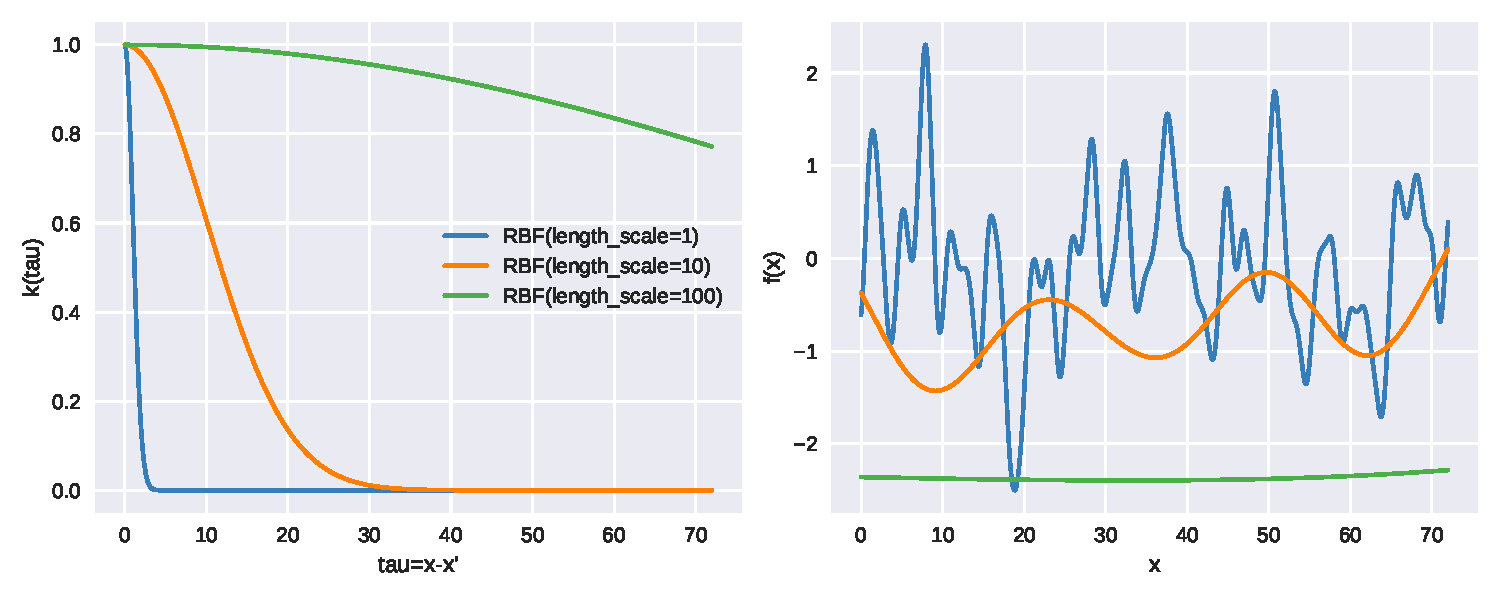
\includegraphics[width=\textwidth]{RBF_length_scale} %<< no file extension
    \caption[RBF Kernel: Kernel function wiht sample path]%<<-- Legend for the list of figures at the beginning of you thesis
   {RBF Kernel function for different length scale (left panel) and a sample
    generate by such a GP (right panel)}
    \label{fig:rbf}
\end{figure}


\subsection{The Matérn Class of Kernel Functions}

An expression for the Matérn covariance function is given by:

\begin{gather*}
    k_{\nu}(\tau) = \frac{2^{1-\nu}}{\Gamma(\nu)}(\frac{\sqrt{2\nu} \tau}{l})^{\nu} K_{\nu}
    (\frac{\sqrt{2\nu} \tau}{l})
\end{gather*}
where $\nu$ and $l$ are positive parameters and $K_{\nu}$ is a modified Bessel
function. The Matérn covariance function and corresponding sample path for different
$\nu$ are shown in figure \ref{fig:matern}.

For $\nu = r + 1/2, r \in \mathbb{N}$ the expression for the Matérn covariance
function can be simplified to:

\begin{gather}\label{kernel-matern}
    k_{\nu=r+1/2}(\tau) = \exp(-\frac{\sqrt{2r + 1} \tau}{l}) \frac{r!}{(2p)!}
    \sum_{i=0}^{r} \frac{(r+i)!}{i!(r-i)!}(\frac{2 \sqrt{2 r + 1} \tau}{l})^{r-i}
\end{gather}

\begin{figure}[!hbt]%--- Picture 'H'ere, 'B'ottom or 'T'op; '!' Try to
                    %impose your will to LaTeX
  \centering
  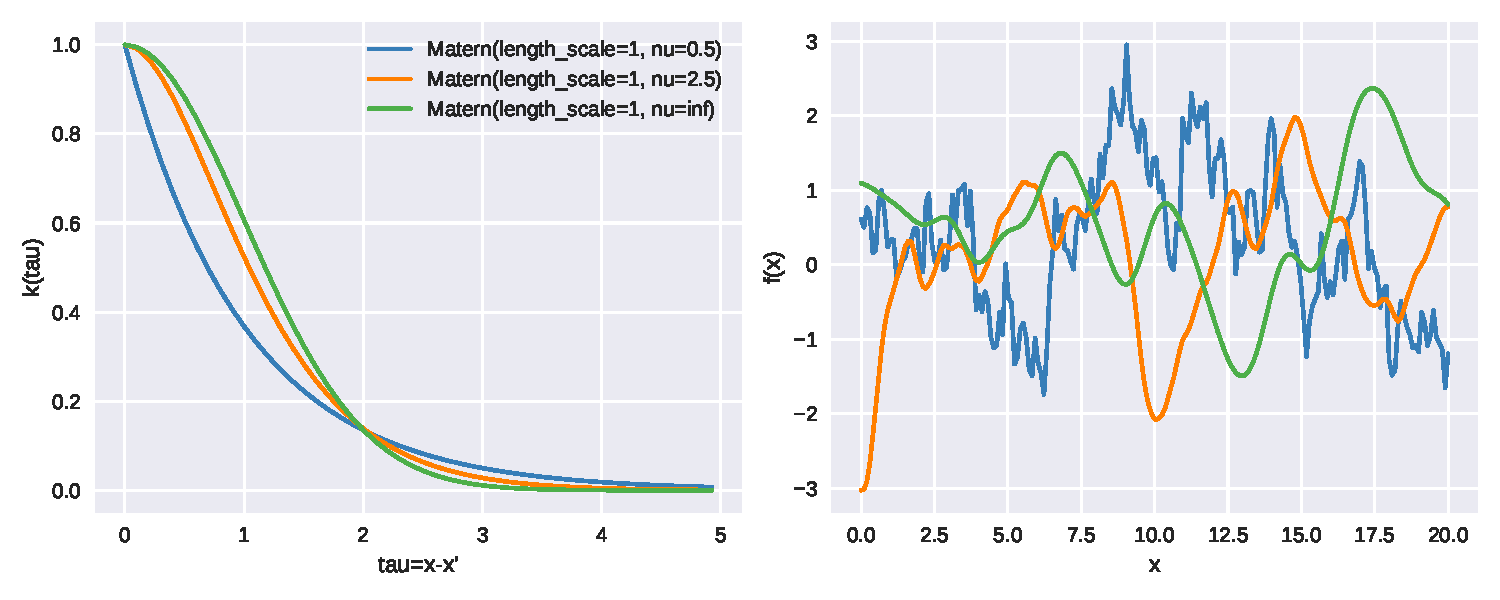
\includegraphics[width=\textwidth]{Matern_nu} %<< no file extension
  %%         --- .5\textwidth stands for 50% of text width
  \caption[Matérn Kernel: Kernel function wiht sample path]%<<-- Legend for the list of figures at the beginning of you thesis
   {Matérn kernel function for different $\nu$ (left panel) and a sample
    generate by the corresponding GP (right panel)}
  \label{fig:matern}
\end{figure}


Setting $\nu = 1/2$ with input domain $X \subset \mathbb{R}$ gives raise to a continuous-time AR(1) process,
also called Ornstein-Uhlenbeck process.
With $\nu = 1/2$, i.e. $r=0$, the Matérn covariance function is given by:
\begin{gather}\label{kernel-matern-ar1}
    k(\tau) = exp(- \tau/l)
\end{gather}
More generally, for $\nu = p - 1/2$ and $X \subset \mathbb{R}$ the Matérn kernel
matches the covariance function of a particular case of continuous AR(p) process.
For further details on this matter
see chapter 4 from the Book of \citeauthor{rasmussen_gaussian_2006}.

%and for more on the Ornstein-Uhlenbeck process see section \ref{app:ou}.

\subsection{The Periodic Kernel Function}

A periodic kernel allows to model functions that feature a repeating pattern
and has the following form:

\begin{gather*}
k(x, x') = \sigma^2 \exp(- \frac{2 \sin^2(\pi |x-x'| \backslash p)}{l^2})
\end{gather*}

where $p$ is the period, and $l$ is the length scale.
The impact of different length scales are illustrated in figure \ref{fig:periodic}.

\begin{figure}[!hbt]%--- Picture 'H'ere, 'B'ottom or 'T'op; '!' Try to
                    %impose your will to LaTeX
  \centering
  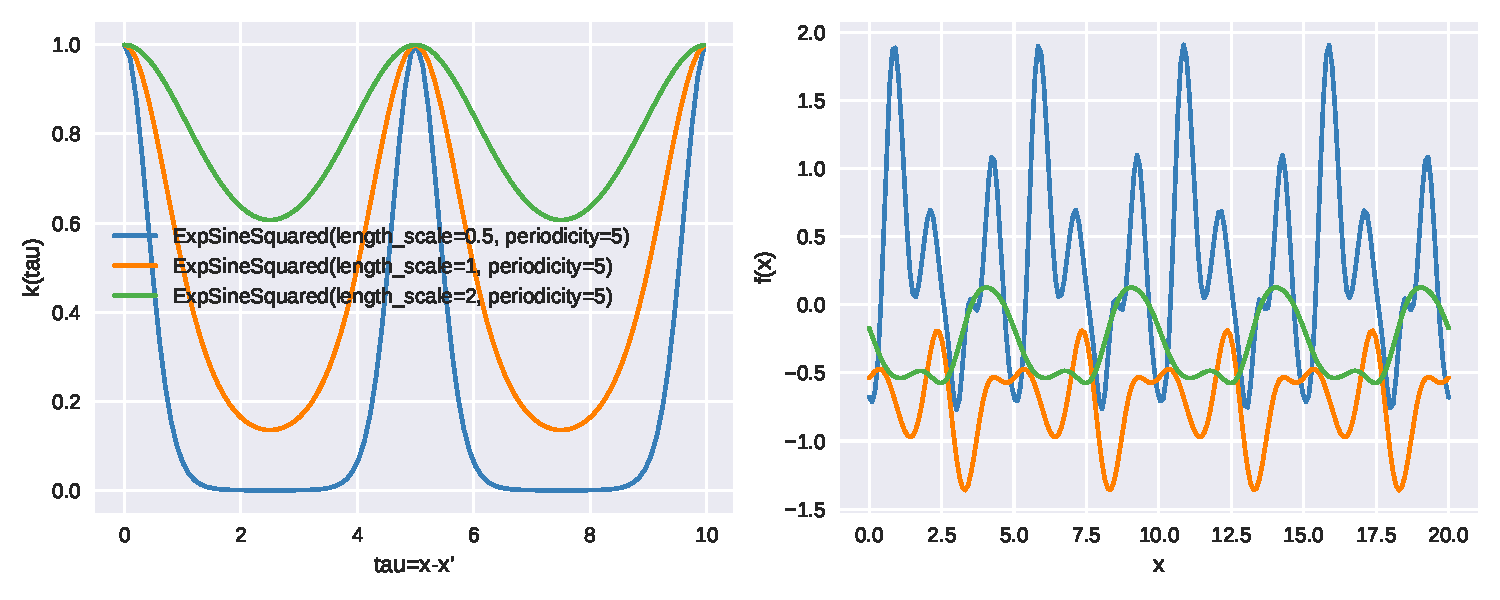
\includegraphics[width=\textwidth]{ExpSineSquared_length_scale} %<< no file extension
  %%         --- .5\textwidth stands for 50% of text width
  \caption[Periodic Kernel: Kernel function wiht sample path]%<<-- Legend for the list of figures at the beginning of you thesis
   {Periodic kernel function for different length scales (left panel) and a sample
    generate by the corresponding GP (right panel)}
  \label{fig:periodic}
\end{figure}



\subsection{Additive Kernels and Decomposition of Predictive Mean}

Additivity of the kernel implies additivity of the predictive mean.
For instance if we choose $Y(x) \sim GP(0, k(x,x'))$ with $k(x,x') = k_1(x, x') + k_2(x,x')$, then
the predictive (posterior) mean $\bar{\mu}(x^{\ast})$
is given by:
\begin{align*}
    \bar{\mu}(x^{\ast}) &= (K_{1, x^{\ast}X} + K_{2, x^{\ast}X}) (K_{XX})^{-1} \mathbf{Y}
    = K_{1, x^{\ast}X} (K_{XX})^{-1} \mathbf{Y} + K_{2, x^{\ast}X}) (K_{XX})^{-1} \mathbf{Y} \\
    &= \bar{\mu}_1(x^{\ast}) + \bar{\mu}_2(x^{\ast})
\end{align*}

where:
\begin{gather*}
    K_{1, x^{\ast}X} =
    \begin{bmatrix}
        k_1(x_1, x^{\ast}) & \dots & k_1(x_n,  x^{\ast})
    \end{bmatrix}, \\
    K_{2, x^{\ast}X} =
    \begin{bmatrix}
        k_2(x_1, x^{\ast}) & \dots & k_2(x_n,  x^{\ast})
    \end{bmatrix},
\end{gather*}
and
\begin{gather*}
        K_{XX} =
    \begin{bmatrix}
        k(x_1, x_1) & \dots & k(x_1, x_n)\\
        \vdots  &  & \vdots \\
        k(x_n, x_1) & \dots  & k(x_n, x_n)
    \end{bmatrix}
\end{gather*}

This decomposition allows us to study
the contribution of the different (additive) kernel components on the predictive mean function.


\section{Performance Assessment}\label{sec:performance-assessment}
Inference, in the case of Gaussian process regression, revolves around the posterior (predictive) distribution
of the response variable.
To evaluate how effectively the predictive distribution explains the observed values
$\mathbf{y^{\ast}}$,
it is common practice to calculate the probability of these values based on the predictive distribution.
Equation \ref{eq:posterior-gp-noise} presents an expression for the predictive distribution of
$\mathbf{Y^{\ast}}:= [Y(x_1^{\ast}), \dots, Y(x_k^{\ast})]^{\top}$ at arbitrary inputs
$X^{\ast} = [x_1^{\ast}, \dots, x_k^{\ast}]$.
Expanding the expression from \ref{eq:posterior-gp-noise} we obtain:

\begin{gather}\label{eq:predictive-dist}
    \log p(\mathbf{Y^{\ast}} = \mathbf{y^{\ast}}| \mathbf{Y}, X) =
    -\frac{k}{2} \log 2 \pi - \frac{1}{2} \log|\bar{\Sigma}| -
        \frac{1}{2}(\mathbf{y^{\ast}} - \bar{\mu})^{\top} \bar{\Sigma}^{-1} (\mathbf{y^{\ast}} - \bar{\mu})
\end{gather}
where
$\bar{\Sigma} = K_{X^{\ast}X^{\ast}} - K_{X^{\ast}X} K_{XX}^{-1} K_{XX^{\ast}}$
and $\bar{\mu} = K_{X^{\ast}X} K_{XX}^{-1} \mathbf{Y}$.

The higher the log probability, the better the fit to the data.
In contrast to other performance metrics it accounts for the complete predictive
distribution rather than just a point estimate.
For instance, when employing the sum of squared errors between the true values $y^{\ast}$ and the predictive mean
$\bar{\mu}$, the predictive covariance matrix $\bar{\Sigma}$ is completely ignored.

\section{Model Selection}

Model selection in Gaussian process regression involves identifying the optimal covariance function
along with the optimal hyperparameters.
Two common approaches for model selection are cross-validation, using a performance-based loss
function as discussed in Section \ref{sec:performance-assessment}, and Bayesian model selection,
which will be explored in the subsequent subsections.
The concepts and ideas discussed in this section are primarily derived from Chapter 5 of
the textbook from \citeauthor{rasmussen_gaussian_2006}.

\subsection{Bayesian Model Selection}

Bayesian model selection aims to find the most probable model given the available data
using a hierarchical specification of the model.
In a parametric model setting, the lowest level consists of the parameters $\beta$,
followed by the hyperparameters $\theta$, which control the parameter distribution.
The highest level encompasses the set of possible model structures $M_i$.

The posterior distribution over the parameters $\beta$ is determined using Bayes' rule:
\begin{gather*}
    p(\beta | \mathbf{Y}, X, \theta, M_i) = \frac{p( \mathbf{Y}| X, \beta,
        M_i)p(\beta|\theta, M_i)}{p(\mathbf{Y}|X, \theta, M_i)}
\end{gather*}

Here, $p(\mathbf{Y} | X, \beta, M_i)$ represents the likelihood, $p(\beta | \theta, M_i)$ denotes the prior,
and $p(\mathbf{Y} | X, \theta, M_i)$ represents the marginal likelihood.


However, in the non-parametric setting of Gaussian processes, the parameter $\beta$ does not exist and is
replaced by the function $f$ itself.
Consequently, at the lowest level, the distribution over the function $f$ is modeled using a Gaussian process.
Similarly to the parametric setting, the posterior distribution over the function values
$f^{\ast} = f(x^{\ast})$ at some arbitrary input $x^{\ast}$ is given by:
\begin{gather*}
    p(f^{\ast} | \mathbf{Y}, X, \theta, M_i) = \frac{p( \mathbf{Y}| f^{\ast}, M_i)p(f^{\ast} | \theta, M_i)}{p(\mathbf{Y}|X, \theta, M_i)}
\end{gather*}

This is equivalent to the expression in \ref{eq:posterior-gp} for the posterior distribution over the
function values $f^{\ast}$ when assuming a Gaussian process prior $f \sim GP(0, k(x,x'))$.
However, in the equation above, $k(x,x')$ is expressed through $\theta$ and $M_i$.

By assuming a prior distribution over the hyperparameters $\theta$, a similar expression can be obtained for
the posterior distribution over the hyperparameters:
\begin{gather*}
    p(\theta | \mathbf{Y}, X, M_i) = \frac{p( \mathbf{Y}| X,M_i, \theta)
        p(\theta| M_i)}{p(\mathbf{Y}|X, M_i)}
\end{gather*}
Maximizing $p(\theta | \mathbf{Y}, X, M_i)$ yields the optimal hyperparameters.
However, when non-Gaussian priors are assumed for $\theta$, evaluating $p(\theta | \mathbf{Y}, X, M_i)$
can be challenging.
In such cases, it is common to maximize the marginal likelihood $p(\mathbf{Y} | X, \theta, M_i)$
with respect to the hyperparameters $\theta$.
This approach is equivalent to assuming uniform distributions over the hyperparameters.
The next subsection will provide more details on how to calculate and maximize the
marginal likelihood for Gaussian process regression.

Note that the scheme mentioned above can be extended to maximize the posterior over the model structures
$M_i$ in order to determine the optimal model structure.
In Gaussian process regression, this corresponds to finding the optimal kernel function type.
However, instead of directly evaluating the posterior, it is often achieved through simultaneous optimization of
the marginal likelihood with respect to the model structure $M_i$ and its hyperparameters $\theta$.
By jointly optimizing these components, we can effectively identify the most suitable kernel function for
the given problem.



%The posterior distribution over the model $M_i$ is given by:
%\begin{gather*}
%    p(M_i | \mathbf{Y}, X) = \frac{p( \mathbf{Y}| X)
%        p(M_i)}{p(\mathbf{Y}|X)}
%\end{gather*}
%where $p(\mathbf{Y}|X) = \sum_i p(\mathbf{Y}|X, M_i)p(M_i)$


\subsubsection{Marginal Likelihood}

In the context of Bayesian linear regression, the marginal likelihood expression was previously
introduced in subsection \ref{subsec:bayesian-linear-regression},
assuming a prior distribution of $p(\beta) = \mathcal{N}(0, \Sigma_p)$ and a likelihood function of
$p(\mathbf{Y} | X, \beta) = \mathcal{N}(X \beta, \Sigma_r)$.
The following expression for the marginal likelihood is obtained by marginalizing over $\beta$:

\begin{gather}\label{eq:marginal-likelihood2}
    p(\mathbf{Y}|X) = \int p(\mathbf{Y}|X,\beta) p(\beta) d\beta = \N(0, X \Sigma_p X^{\top} + \Sigma_r)
\end{gather}

Furthermore, as discussed in section \ref{sec:gaussian-process-regression},
the marginal likelihood can also be represented as a distribution over the function $Y(x)$:
\begin{gather*}
    Y(x) \sim GP(0, k(x, x'))
\end{gather*}
Here, the kernel function $k(x, x')$ is chosen such that for an index set $X$,
we obtain $K_{XX} = X \Sigma_p X^{\top} + \Sigma_r$.

By the definition of a Gaussian process, $\mathbf{Y}|X$ follows a multivariate normal distribution
with a covariance matrix of $K_{XX}(\theta)$, which is a function of the hyperparameters $\theta$.
The log marginal likelihood is hence given by:
\begin{gather}\label{eq:gaussian-marginal-likelihood}
    \log p(\mathbf{Y} | X, \theta) = - \frac{1}{2} \mathbf{Y}^{\top} K_{XX}^{-1}(\theta) \mathbf{Y} -
    \frac{1}{2} \log |K_{XX}(\theta)| - \frac{n}{2} \log 2 \pi
\end{gather}

Since the marginal likelihood already incorporates a trade-off between model fit and
model complexity, it is a suitable candidate for solving the model selection problem.
The first term, $- \frac{1}{2} \mathbf{Y}^{\top} K_{XX}^{-1}(\theta) \mathbf{Y}$,
represents a measure of the data fit. The second term, $\frac{1}{2} \log |K_{XX}(\theta)|$,
penalizes more complex models. The last term $\frac{n}{2} \log 2 \pi$ serves as a normalization constant.















